Trabaje para $t\ge0$ con la transformada unilateral de Laplace y entradas causales. Use $H(t-a)=0$ para $t<a$ y $H(t-a)=1$ para $t\ge a$; los valores aislados en saltos no alteran la transformada. Sean $a,b,h>0$. Las gráficas definen el pulso $f$ y la sucesión $g$, que alterna el signo de pulsos consecutivos sin intervalo entre ellos y continúa indefinidamente. Los lados oblicuos son rectos y $L=2a+b$.
\begin{center}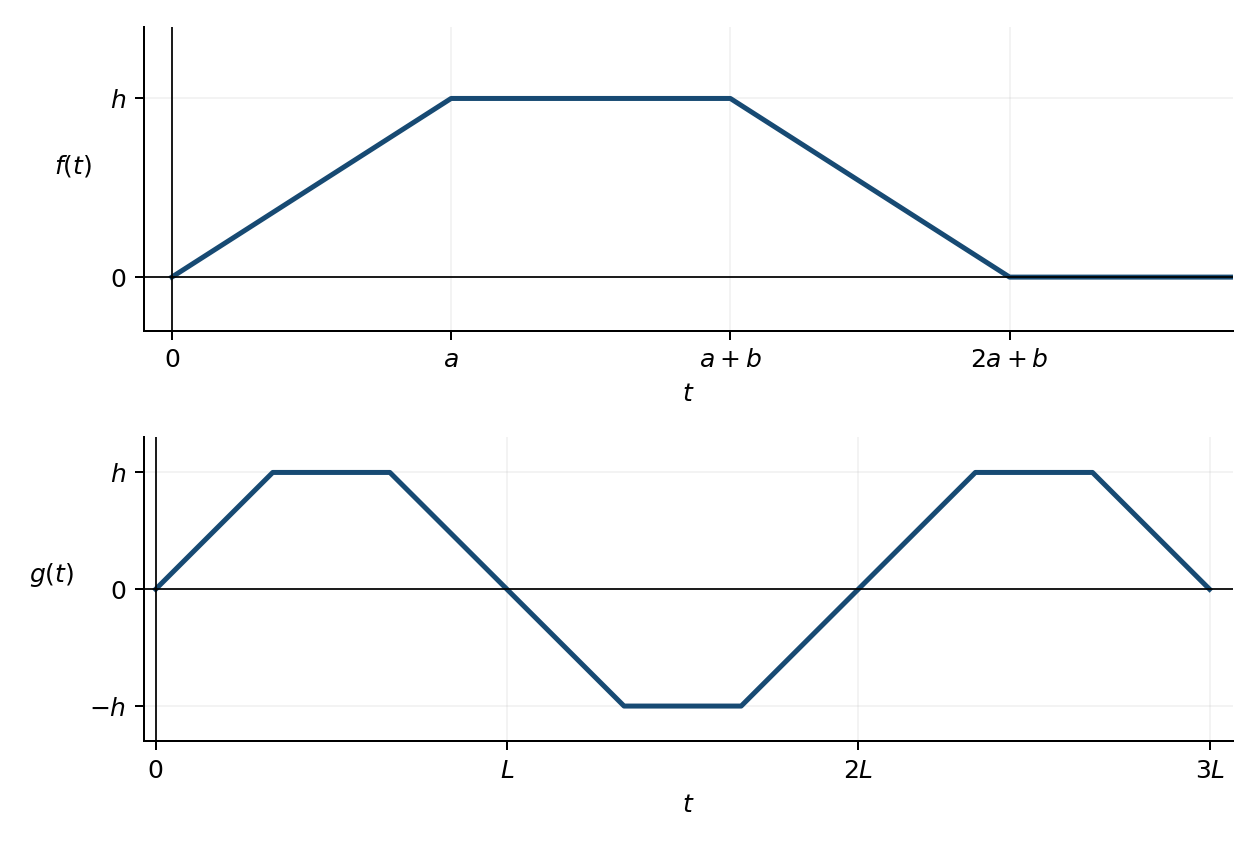
\includegraphics[width=.95\linewidth]{assets/M2-E0226-inputs.png}\end{center}

\begin{enumerate}[label=(\alph*),ref=\alph*,leftmargin=*]
\item Calcule la transformada de $f$.
\item Calcule la transformada de $g$.
\item Para $a=b=h=1$, resuelva $y'+y=g(t)$, $y(0)=0$.
\end{enumerate}
